\chapter{Literature Review}
\label{cha:Literature Review}

\section{Car Following Models}
\label{sec:Car Following Models}
Any autonomous-vehicle system will implement a `car-following model', which defines actions for a vehicle based on the behaviour of its predecessors (the vehicles in front of it). One early car-following model was defined in 1981 by P.G. Gipps \citep{Gipps1981}. It was designed to mimic real-world driver behaviour, calculating a safe travelling speed for a vehicle based on the speed of its predecessor. A safe travel speed is defined as a speed at which the driver can safely stop if the preceding driver stops.

Gipps defined two equations applying constraints on the acceleration and braking profiles of the vehicles. Appendix \ref{subsec:Gipps 1981 Equations} details these equations. Gipps' model worked well at describing the behaviour of traffic. However, translating this work to autonomous vehicles poses a number of problems. Firstly, the work is based on the behaviour of real-world drivers in instrumented vehicles. This introduces human driver variables into the equations. Gipps' modelled reaction time, which will be far smaller for autonomous vehicles. The gaps between successive vehicles are also larger than necessary. Autonomous vehicles are more precise than human drivers and can drive closer to their predecessors. Gipp's model also focuses solely on single-lane drivers.

In 2000 Treiber et al. suggested the `Intelligent Driver Model' (IDM) \citep{Treiber2000}. This model, detailed further in Appendix \ref{subsec:The Intelligent Driver Model}, defines an acceleration profile for a vehicle as a continuous function. This function is based on the vehicle's current velocity, its desired velocity and the distance from the vehicle to its successor.

The IDM does not attempt to directly mimic human behaviour in traffic situations. It models a general acceleration and braking profile for a given vehicle. As such, it is well suited for adaptation by autonomous vehicle models, as seen in Kesting's work \citep{Kesting2007} in Section \ref{subsec:Lane Changing to improve overall velocity}. However, similarly to Gipps' model, it solely focuses on single-lane drivers.

Gipps' model and the IDM also both fail to recognise, and incorporate, the use of vehicle-to-vehicle communication in their models. Autonomous vehicles could communicate with each other to help reduce overall travel time and improve efficiency. In vehicle platoons, such as those analysed by Kamali in 2016 \citep{Kamali2016}, each vehicle autonomously follows it's predecessor, with the lead vehicle controlling the overall pace of the platoon. Platoons make heavy use of vehicle-to-vehicle (V2V) communication to allow vehicles to join and leave, as well as to continuously control vehicle spacing and velocity. The advantage of a platoon is that all vehicles can accelerate and decelerate simultaneously reducing the effect of traffic shocks \citep{Daganzo1994}.

\section{Centralised and Decentralised}
\label{sec:Centralised and Decentralised}
We can divide approaches to autonomous vehicles into centralised and decentralised solutions. Centralised solutions rely on an external agent to manage vehicles. Vehicles use vehicle-to-infrastructure (V2I) communication channels to send information and receive instructions from the external agent. Decentralised solutions use vehicle-to-vehicle (V2V) communication to let other vehicles know their state, their intentions and to arrange any complex actions that might affect surrounding vehicles.

\subsection{Centralised Systems}
\label{subsec:Centralised Systems}
The Autonomous Intersection management system (AIM) described in \citep{Dresner2004} is an example of a centralised V2I system. The system works by dividing the intersection into a grid of $n \times n$ reservation tiles. Drivers `call ahead' to the intersection sending information packets containing

\begin{enumerate}
\item The time the vehicle will arrive.
\item The velocity at which the vehicle will arrive
\item The direction the vehicle will be facing when it arrives
\item The vehicle's maximum velocity
\item The vehicle's maximum and minimum acceleration
\item The vehicle's length and width
\end{enumerate}

The intersection infrastructure simulates the journey of the vehicle through the intersection, noting the tiles occupied by the vehicle at each time interval. If any cell is reserved at the same time step the intersection rejects the request. The driver will start decelerating and continue making requests until it obtains a reservation. It will not enter the intersection without a reservation, even if that means coming to a stop at the intersection.

\begin{figure}[htb]
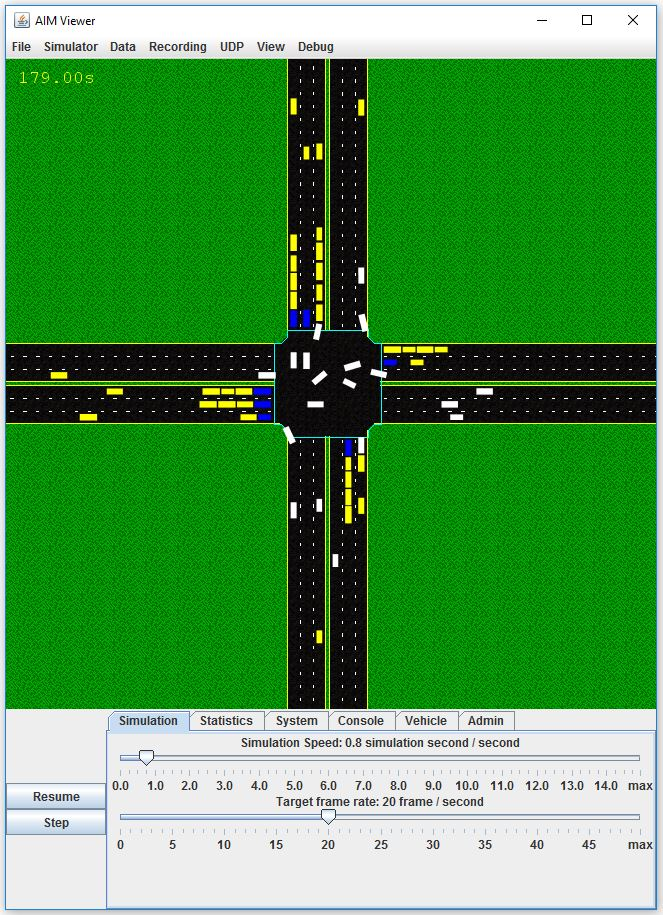
\includegraphics[width=\textwidth]{litReview/aimOriginal.JPG}
\caption{Screenshot of the AIM Simulator}
\label{fig:AIMOriginal}
\end{figure}

A grid-based reservation system works well in high traffic zones like intersections, because it forces all vehicles to communicate with a single entity. This entity has a global-view of activity at the junction, allowing the system to make vehicle management decisions more easily. A V2V solution would require more complex communication protocols involving large numbers of vehicles. The volume of messages required for each vehicle to obtain a global view of the intersection would be considerably larger, and as such, most vehicles will never get a complete understanding of the status of the intersection.

This paper forms the foundation for the AMM protocol designed in Section \ref{sec:Autonomous Merge Management System}.

\FloatBarrier
\subsection{Decentralised Systems}
\label{subsec:Decentralised Systems}
The main arguments against centralised systems generally tend to stem from concerns over feasibility and fault tolerance. A centralised V2I solution relies on one system always being available to manage vehicles. The original implementation of the AIM system works well, but if the system were to fail and no longer provide reservations, then approaching vehicles will simply halt at the intersection. In a worst case scenario, the system would still give reservations, but fail to compare them to reservations already in place, causing major car crashes in the intersection. Having, a single point of failure like this is a major concern, particularly when lives are on the line.

A paper by VanMiddlesworth et al. in 2008 \citep{VanMiddlesworth2008} defined a decentralised version of the AIM model using V2V communication protocols. In VanMiddlesworth's model each vehicle can broadcast two different types of message. These messages are broadcast repeatedly with a specified period.
\begin{enumerate}
\item \emph{Claim}
This is a message indicating the vehicle's intention to traverse the intersection. It provides the vehicle's VIN, arrival lane, turning direction, arrival time and exit time. It also provides a message id, which increments when a new message is broadcast. Finally, the \emph{Claim} message contains a boolean indicating whether the vehicle has stopped at the intersection.
\item \emph{Cancel}
This message releases any currently held reservation, it contains the vehicle's VIN and a message id, which acts the same as the message id in \emph{Claim}.
\end{enumerate}

Two \emph{Claim} messages are in conflict if their paths, as determined by their lane and turn parameters, are incompatible and their time intervals, as determined by their arrival and exit times, overlap. To resolve the conflict VanMiddlesworth's model determines which Claim has dominance. A claim $C_1$ dominates another claim $C_2$ if $C_1$'s vehicle is stopped at the intersection and $C_2$'s vehicle is not. If $C_1$ and $C_2$ both have the same value for the stopped at intersection boolean, dominance is determined based on priority. Priority is indicated by the following rules, given in order of evaluation:
\begin{enumerate}
\item If neither vehicle is stopped at the intersection, the claim with the earliest exit time has priority.
\item If both vehicles are stopped, the vehicle whose lane is 'on the right' has priority. This is defined similarly to current US 4-way stop rules.
\item If neither lane can be considered to be on the right the vehicle who is not making a turn has priority.
\item If no other priority order can be established, the vehicle with the lowest VIN has priority.
\end{enumerate}

The protocol starts with approaching vehicles receiving messages from existing pending vehicles. An approaching vehicle may not start broadcasting it's own messages until it is within 'lurk distance' of the intersection. 

Once within lurk distance the vehicle generates a \emph{Claim} message for the earliest possible time the vehicle might arrive at the intersection. Once the vehicle has a \emph{Claim} broadcasting it may need to change it if it's looking like the vehicle might be late to the intersection or if a competing \emph{Claim} dominates it. A vehicle might also change its \emph{Claim} to take advantage of a newly available time slot. In this situation the vehicle must then send a \emph{Cancel} message and a new \emph{Claim}. The \emph{Cancel} message is sent repeatedly with the same period as the \emph{Claim} message. Once the vehicle reaches the intersection it must traverse according to its current \emph{Claim}, broadcasting its \emph{Claim} throughout the traversal. At this point, the vehicle's claim cannot be dominated.

The main drive behind the unmanaged AIM intersection was to reduce cost. Adding in new infrastructure to an intersection costs money, and it might not be considered worthwhile for small intersections with only one or two lanes on each side. An unmanaged, decentralised system like that described by VanMiddlesworth would drastically reduce the cost to the state in creating automated road networks.

This paper forms the foundation for the decentralised protocol designed in Section \ref{sec:Decentralised Merge Management System}.

\section{Making lane changing decisions}
\label{sec:Making lane changing decisions}
Lane changes are a form of lane merging, in which the lanes are parallel. Some of the lane merging approaches here could help in designing merge protocols. It could also help when it comes to dealing with multi-lane merges.

There are a number of reasons that a driver would want to change lanes. The most obvious being that the journey the driver wishes to complete requires the vehicle to move into a different lane. In this case the vehicle \emph{must} change lanes before it reaches a critical position. Beyond this position the driver will need to change their planned route, most likely extending their journey time. 

Another reason a driver might change lanes is in order to increase velocity, with the aim of reducing journey time. In general, a driver will aim to change lanes if their average velocity in their current lane is much less than that the velocity it could be achieving in another lane.

\subsection{Lane Changing to hit a target lane}
\label{subsec:Lane Changing to hit a target lane}
In 2016 Atagoziyev et al. described a centralised system for lane changes \citep{Atagoziyev2016}. This system uses roadside infrastructure to help groups of vehicles change lanes before they reach a `critical-position', such as a motorway exit or intersection. The vehicles send their position and velocity information to the roadside infrastructure. The system keeps track of the gaps between vehicles and their relative speeds, and then uses a series of equations to determine how to manipulate a vehicle into its desired land. Each equation is used in a different context, based on the relative positions of surrounding vehicles. With the context identified, the system uses a finite state automata to determine the instructions to send to the vehicle. The set of contexts Atagoziyev's system deals with, and the actions taken for each one can be found in Appendix \ref{sec:Atagoziyev's Model}.

Atagoziyev's model forces cooperation between vehicles by forcing them to move out of each others way in order to allow vehicles to reach their target lanes. This is far better than human drivers who have no requirement to act selflessly during lane changes. However, Atagoziyev's model does suffer from being a centralised system and cannot be applied to situations far from critical-positions. As most merges will be at `critical-positions' however, this matters less to our problem. A simple merge system that forces vehicles to take turns and allow others to pass through could work as well as Atagoziyev's model, which proved to be effective in multiple lane change scenarios.

\subsection{Lane Changing to improve overall velocity}
\label{subsec:Lane Changing to improve overall velocity}
Work by Kesting et al. in 2007 \citep{Kesting2007} describes a decentralised model of lane changing that lets vehicles change lanes to increase velocity whilst still ensuring that the overall traffic flow is not disrupted. This helps to avoid traffic shocks and maintains smooth traffic flow. In order to do this, Kesting introduces the MOBIL or `Minimising Overall Braking Induced by Lane Changes' model, which is further detailed in Appendix \ref{subsec:The MOBIL Model}. 

The model uses two criterion that the vehicle must satisfy. The first gives the vehicle a maximum deceleration value. The second is the `incentive criterion', the motivation for a driver to change lanes. Whether a driver changes lanes or not is based on the relationship between the utility a driver gets by changing lanes, and the utility the vehicle behind the driver in the new lane loses by being pulled out in front of. How willing a driver is to sacrifice another driver's utility for their own is down to the driver's politeness factor $p$. With a $p$ value of 0, drivers act selfishly, with no regard for the utility of other drivers. With a $p$ value of 1, drivers act altruistically, only changing lanes when it has a net benefit to all drivers involved, at least above a set threshold. A $p$ value of 1 also caused the maximum lane changing rate to halve. Kesting also discovered that `altruistic' lane changing behaviour increased the mean speed of both lanes involved in the simulation, improving overall traffic performance.

A modified version of MOBIL could be used to manage merges with slip lanes, with drivers only merging in front of another vehicle when it has the least impact on both drivers. The politeness factor would have to change as the vehicle came closer to the end of the slip lane however, as eventually the vehicle must merge, or suffer a collision. 